%% starts at line 70
\documentclass[twocolumn,linenumbers,trackchanges]{aastex7}
%% \documentclass[argument1,argument2,argument3,...]{aastex7}
%%
%% Six of the arguments are typestting options. They are:
%%
%%  twocolumn: two text columns, 10 point font, single-spaced article.
%%                This is the most compact and represents the final published
%%                derived PDF copy of the accepted manuscript from the publisher
%%  default     : one text column, 10 point font, single spaced (default).
%%  manuscript: one text column, 12 point font, double-spaced article.
%%  preprint    : one text column, 12 point font, single-spaced article.  
%%  preprint2: two text columns, 12 point font, single-spaced article.
%%  modern      : a stylish, single text column, 12 point font, article with
%% 		  wider left and right margins. This uses the Daniel
%% 		  Foreman-Mackey and David Hogg design.
%%
%% Note that you can submit to the AAS Journals in any of these six styles.
%%
%% There are other optional arguments one can invoke to allow other stylistic
%% actions. The available options are:
%%
%%   astrosymb    : Loads Astrosymb font and defines \astrocommands. 
%%   tighten      : Makes baselineskip slightly smaller, only works with 
%%                  the twocolumn substyle.
%%   times        : uses times font instead of the default.
%%   linenumbers: turn on linenumbering. Note, this is mandatory for AAS
%%                  Journal submissions and revisions.
%%   trackchanges: Shows added text in bold.
%%   longauthor: Do not use the more compressed footnote style (default) for 
%%                  the author/collaboration/affiliations. Instead print all
%%                  affiliation information after each name. Creates a much 
%%                  longer author list, but may be desirable for short 
%%                  author papers.
%% twocolappendix: make 2 2-column appendix.
%%   anonymous    : Do not show the authors, affiliations, acknowledgments,
%%                  and author contributions for dual anonymous review.
%%  resetfootnote: Reset footnotes to 1 in the body of the manuscript.
%%                  Useful when there are a lot of authors and affiliations
%%		    in the front matter.
%%   longbib      : Print article titles in the references. This option
%% 		    is mandatory for PSJ manuscripts.
%%
%% Since v6, AASTeX has included \hyperref support. While we have built in 
%% specific %% defaults into the classfile, you can manually override them 
%% with the \hypersetup command. For example,
%%
%% \hypersetup{linkcolor=red,color=green,filecolor=cyan,urlcolor=magenta}
%%
%% will change the color of the internal links to red, the links to the
%% bibliography to green, the file links to cyan, and the external links to
%% magenta. Additional information on \hyperref options can be found here:
%% https://www.tug.org/applications/hyperref/manual.html#x1-40003
%%
%% The "bookmarks" has been changed to "true" in hyperref
%% to improve the accessibility of the compiled PDF file.
%%
%% If you want to create your own macros, you can do so
%% using \newcommand. Your macros should appear before
%% the \begin{document} command.
%%
%% Citation Keys: {GalacticBulges,Besla2012,Querejeta2014,Torrey2012,Hopkins2007,Pardy2016,Kannan2015}
\begin{document}

\title{Galaxy Evolution Through Tidal Interactions:\\Evolution of the Observed and Mass Derived Rotation Curves of M31 and the Milky Way}

\author{Colton Quirk}
\affiliation{University of Arizona}
\email{coltonq@arizona.edu}

%% Mark off the abstract in the ``abstract'' environment. 
%%\begin{abstract}
%%How does the "observed" and mass-derived rotation curve of each galaxy evolve (disk, bulge)? ("Observed" meaning plot the simulated disk particle line of sight velocity field edge on; See Lab 7).
%%\end{abstract}

%% \begin{abstract}

%% \end{abstract}


%% Keywords should appear after the \end{abstract} command. 
%% The AAS Journals now uses Unified Astronomy Thesaurus (UAT) concepts:
%% https://astrothesaurus.org
%% You will be asked to selected these concepts during the submission process
%% but this old "keyword" functionality is maintained in case authors want
%% to include these concepts in their preprints.
%%
%% You can use the \uat command to link your UAT concepts back its source.
\keywords{\uat{Galaxies}{573} --- \uat{Rotation Curve}{619}---\uat{Stellar Disk}{1594} ---\uat{Major Merger} ---\uat{Hernquist Profile} ---}

%% From the front matter, we move on to the body of the paper.
%% Sections are demarcated by \section and \subsection, respectively.
%% Observe the use of the LaTeX \label
%% command after the \subsection to give a symbolic KEY to the
%% subsection for cross-referencing in a \ref command.
%% You can use LaTeX's \ref and \label commands to keep track of
%% cross-references to sections, equations, tables, and figures.
%% That way, if you change the order of any elements, LaTeX will
%% automatically renumber them.

\section{Introduction}
%% Include a figure to support one of the above paragraphs.
%% Need to reference at least 3 papers in the above paragraphs.
%% Define your proposed topic and how it pertains to Galaxy Evolution. You should describe this general area of galaxy dynamics and evolution.
The study of galaxy evolution is crucial to understanding the large-scale structure of the universe and the mechanisms that drive changes in galactic morphology and kinematics.
One key aspect of galaxy evolution is the role of tidal interactions in shaping the observed and mass-derived rotation curves of galaxies.
This project focuses on the evolution of the rotation curves of the Milky Way and M31 (the Andromeda Galaxy), particularly how their disk and bulge components respond to gravitational interactions over time.
Tidal interactions are the gravitational forces which arise from interactions between spatially extended objects, not point-sources \citep{GalacticBulges}.
As the two galaxies move towards each other the parts of the galaxy closest to each other will feel a different amount of gravitational force than the parts of the galaxy farther from each other. This will cause the structure of the galaxies to change.
This project will study how the galaxies change by analyzing the rotation curves of each galaxy, for both the disk stars and the bulge stars.
Rotation curves provide insight into the mass distribution of galaxies, distinguishing between visible and dark matter contributions.
By examining how these curves evolve through tidal interactions, we can gain a clearer picture of the dynamical history of these galaxies and their future trajectories.

%% State why this topic matters to our understanding of galaxy evolution.
Understanding the evolution of rotation curves is fundamental to deciphering how galaxies grow, interact, and redistribute their mass.
The discrepancy between observed and mass-derived rotation curves has been a longstanding issue in astrophysics, offering evidence for dark matter or alternative gravitational theories.
Studying these curves in the Milky Way and M31 allows us to explore how tidal interactions—such as satellite mergers, close encounters, and long-range gravitational influences—reshape the internal dynamics of galaxies \citep{Hopkins2007}.
Since both the Milky Way and M31 are on a collision course, analyzing their past and present rotation curves provides a valuable window into how interactions impact galactic structure, angular momentum distribution, and the overall dark matter profile.

\begin{figure}[ht!]
	\centering
	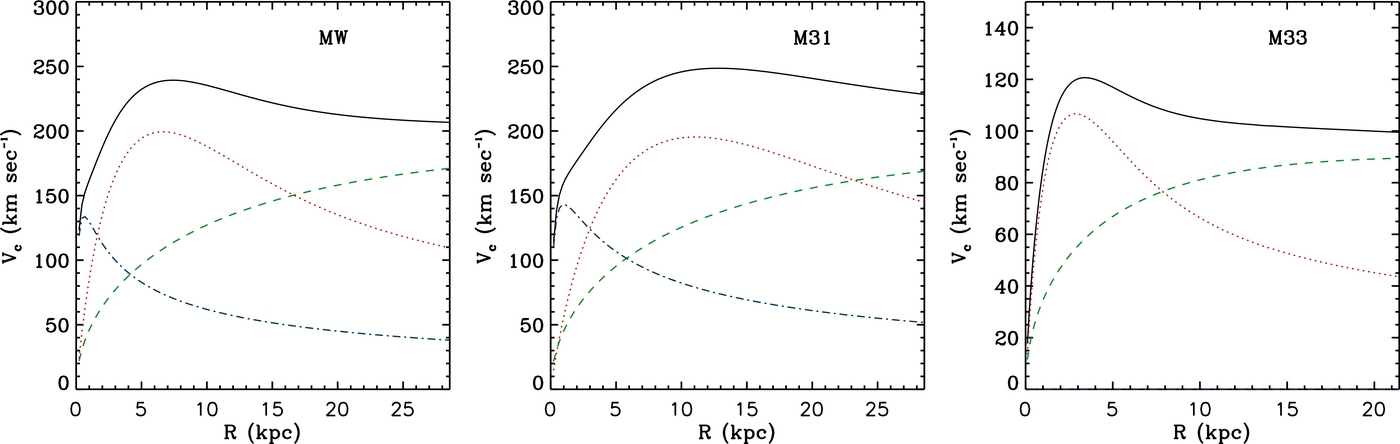
\includegraphics[width=1.0\linewidth]{Rotation_Curves_Besla.jpg}
	\caption{Model rotation curves showing the contributions of the various parts of the galaxies to the rotation curve. This work seeks to create demonstrate the evolution of the rotation curves throughout the first close encounter of M31 and the MW.}
\end{figure}

%% Overview our current understanding of the topic in galaxy evolution, broadly.
Our current understanding of galactic rotation curves stems from both observational and theoretical studies.
Observations of spiral galaxies indicate that their rotation curves remain nearly flat at large radii, implying the presence of extended dark matter halos \citep{GalacticBulges}.
Theoretical models and N-body simulations suggest that tidal interactions can redistribute mass within a galaxy, potentially altering both the baryonic and dark matter components \citep{Besla2012}.
In particular, major interactions, such as mergers or flybys, can lead to angular momentum transfer, bulge growth, and changes in the mass-to-light ratio, all of which impact the rotation curve.

%% What are the open questions related to this topic?
Despite significant progress, many open questions remain regarding the evolution of rotation curves under tidal influences.
How exactly do tidal interactions reshape the mass distribution of the disk and bulge over different timescales \citep{Kannan2015}?
Do observed changes in rotation curves primarily reflect baryonic redistribution, or do they hint at modifications in the dark matter halo?
Additionally, while we can model individual interactions, predicting long-term evolutionary trends remains challenging due to the complex interplay between baryons, dark matter, and external forces.
Finally, as the Milky Way and M31 move toward their eventual merger, how will their respective rotation curves evolve, and what can this tell us about the fate of similar galactic interactions throughout cosmic history?
Addressing these questions will enhance our understanding of galaxy evolution and the nature of dark matter.


\section{This Project}
%% What specific question(s) will you be addressing using the simulation? You only need to pick one - think about how much time you have realistically!
This project seeks to answer how the rotation curves of the Milky Way and the Andromeda galaxy change over time.
For example, do the rotation curves maintain a flat profile throughout the merger?
If they do not maintain a flat profile when and why does it deviate?
As well this project will analyze how the disk and bulge particles within the galaxies are affected by the merger process. 
By answering these questions we can gain significant insights into how mergers affect galaxy evolution.

\section{Methodology}
%% How will you approach the specific question using the simulation data? Define all relevant equations and terms. Here you should outline the codes you'd need to write - each question will need a unique code solution. This can be described in general terms but all steps need to be outlined (including what particle types/properties will you select and how you will select them, specify which snapshots will you use).
%% Must include at least one figure that illustrates the methodology.
This project will analyze the rotation curves of the Milky Way and the Andromeda Galaxy throughout their merger. 
We will use all 802 snapshots for both galaxies using the VLowRes data. For each snapshot, we will construct four rotation curves.
We will create rotation curves for both the disk-type and bulge-type particles, particle types 2.0 and 3.0, respectively.
We will also construct two rotation curves, the mass-derived rotation curve and the "observed" rotation curve, for each particle type.

The mass-derived rotation curves are calculated by taking radial slices of the galaxy and measuring the mass within each slice. Then, we can calculate the velocity needed for a particle to have a circular orbit around that mass at that radial slice.

\begin{equation}
	F=m\overrightarrow{a}=m\frac{v^2}{r}=\frac{GMm}{r^2}
\end{equation}

We can solve this equation for the velocity of a circular orbit.

\begin{equation}
	v_{\text{circ}}=\sqrt{\frac{GM}{r}} \label{eq:vcirc}
\end{equation}

This circular velocity would be calculated for each radial slice by measuring the amount of mass within that radial distance.
See Figure \ref{fig:HW5} for an example of a mass-derived rotation curve of M31.

\begin{figure*}[ht!]
	\plotone{HW5_RotationCurve_M31.png}
	\caption{Mass-derived rotation curve for M31 at snap number 0. This was made for Homework 5.}
	\label{fig:HW5}
\end{figure*}

The "observed" rotation curve is the line-of-sight velocity field when viewed edge-on. This will be constructed for each snapshot for each galaxy and particle type.
This will be made using the same technique as used in Lab 7 of this course. 
That is, we will take the galaxy and rotate it so that its angular momentum is aligned with the z-axis. 
Then, we will plot the particles' velocities versus their x-coordinate (relative to the center of mass of the galaxy) as a 2D histogram. 
This will construct a rotation curve of the galaxy for a particular snapshot. See Figure \ref{fig:Lab7} for an example of an "observed" rotation curve.

\begin{figure}[ht!]
	\plotone{Lab7_RotationCurve.png}
	\caption{"Observed" rotation curve for M31 at snap number 0. This was made for Lab 7.}
	\label{fig:Lab7}
\end{figure}

Thus, the overall process for finding how the rotation curves change over time is shown below.
This process will be completed for both galaxies.
\begin{enumerate}
	\item Load the data for a particular snapshot
	\item Create two MassProfile objects, one for Disk Particles and the other for Bulge Particles
	\item For each MassProfile object, create a mass derived rotation curve using equation \ref{eq:vcirc}
	\item For each MassProfile, rotate the frame of the galaxy such that the angular momentum aligns with the z-axis
	\item Then plot the x-coordinate versus the velocity of the particles as a 2D histogram
	\item Save both of these profiles and continue to the next snapshot
\end{enumerate}

These rotation curves will then be overplotted to show how the "observed" and mass-derived rotation curves align.
The rotation curves will then be added to an animation to show the evolution over time for both galaxies and particle types.


\begin{figure}[ht!]
	\centering
	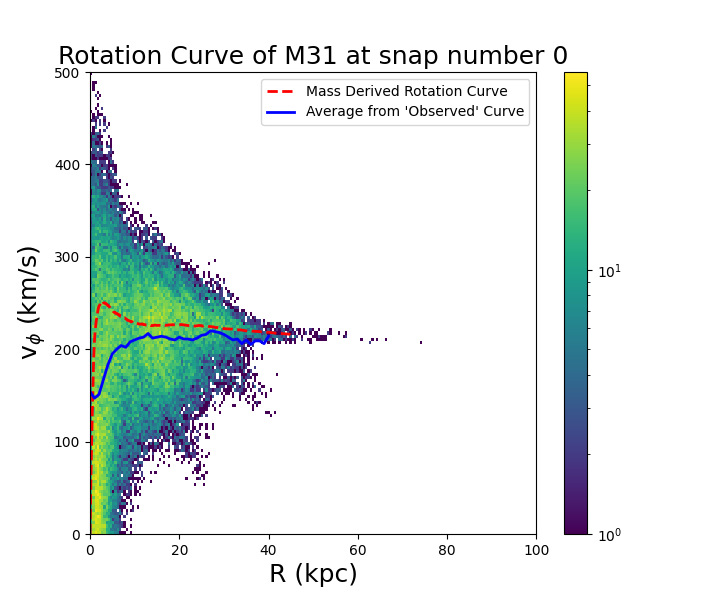
\includegraphics[width=1.0\linewidth]{M31_000_rotation_curve.png}
	\caption{Initial rotaiton curve.}
\end{figure}

\begin{figure}[ht!]
	\centering
	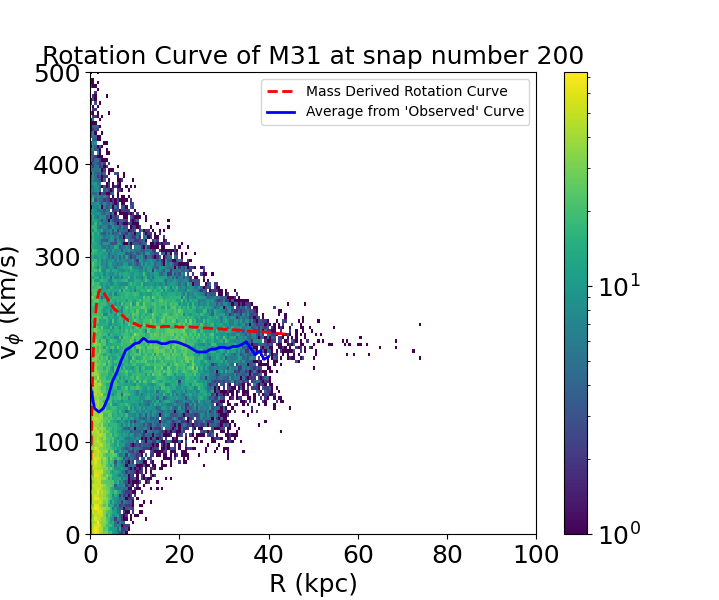
\includegraphics[width=1.0\linewidth]{M31_200_rotation_curve.png}
	\caption{Rotation curve before close encounter.}
\end{figure}

\begin{figure}[ht!]
	\centering
	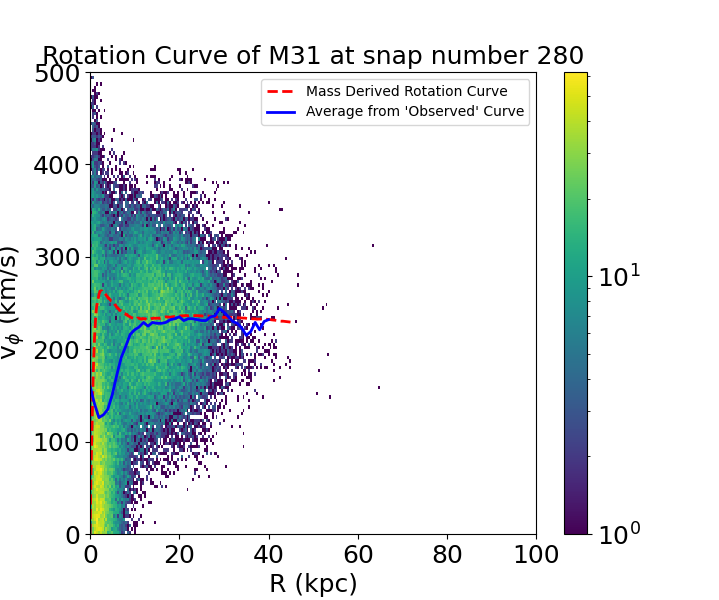
\includegraphics[width=1.0\linewidth]{M31_280_rotation_curve.png}
	\caption{Rotation curve during close encounter.}
\end{figure}

\begin{figure}[ht!]
	\centering
	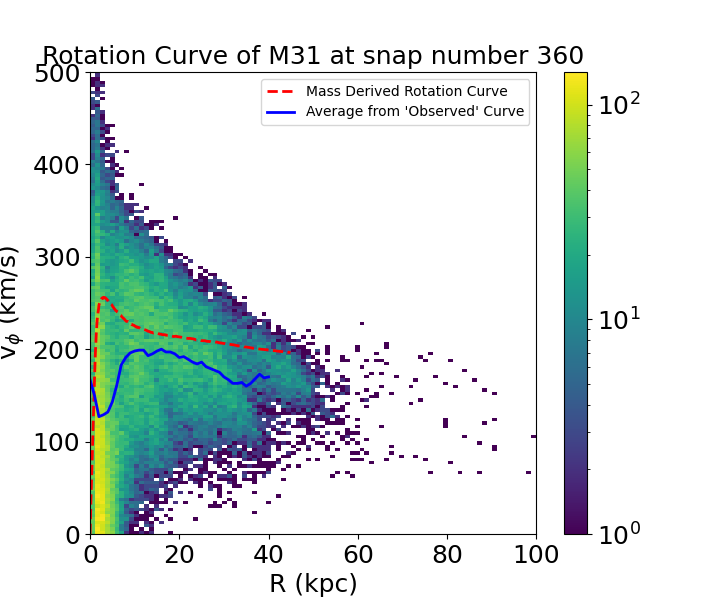
\includegraphics[width=1.0\linewidth]{M31_360_rotation_curve.png}
	\caption{Rotation curve after close encounter.}
\end{figure}

\begin{figure}[ht!]
	\centering
	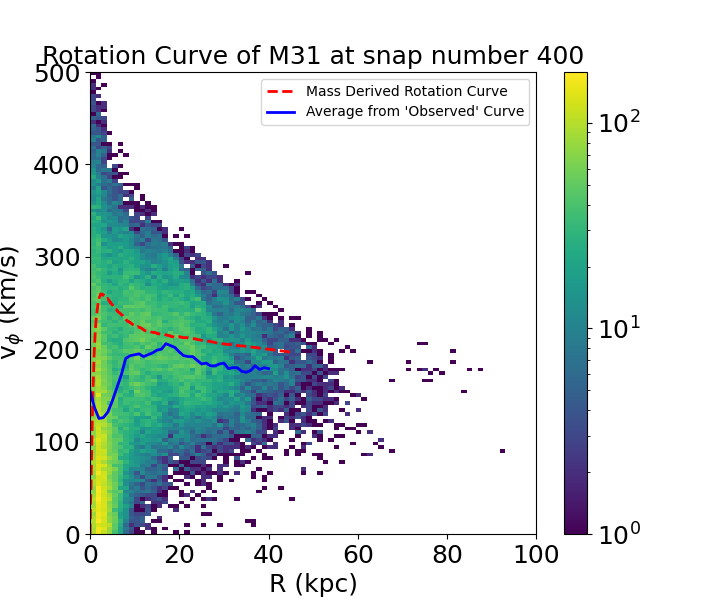
\includegraphics[width=1.0\linewidth]{M31_400_rotation_curve.png}
	\caption{Rotation curves greatly separated from the close encounter.}
\end{figure}

\subsection{Hypothesis}
%% What is your hypothesis for what you will find? Why do you think this will occur?
We hypothesize that the rotation curves will not maintain a flat profile throughout the merger.
As the tidal forces disrupt the rotation of the galaxies, the rotation curves will be impacted.
We also expect there to be some transfer between the rotation curves of the disc particles and bulge particles.
As discussed in \cite{Kannan2015}, there is a transfer of particles between the disc and the bulge of galaxies during mergers.
This will affect the distribution of the galaxies' angular momentum during the merger, leading to variances in the rotation curves of the disc and bulge particles.

%% The "ht!" tells LaTeX to put the figure "here" first, at the "top" next
%% and to override the normal way of calculating a float position.
%% The asterisk after "figure" tells the compiler to span multiple columns
%% if a two-column style is selected.
%% Please use the acknowledgment and contribution environments. This will 
%% be anonymized when the "anonymous" style option is used. 

%%\begin{acknowledgments}
%%\end{acknowledgments}

%% For this sample, we use BibTeX plus aasjournalv7.bst to generate the
%% the bibliography. The sample7.bib file was populated from ADS. To
%% get the citations to show in the compiled file, do the following:
%%
%% pdflatex sample7.tex
%% bibtext sample7
%% pdflatex sample7.tex
%% pdflatex sample7.tex

\bibliography{QUIRK_ResearchAssignment4}{}
\bibliographystyle{aasjournalv7}

%% Include this line if you are using the \added, \replaced, \deleted
%% commands to see a summary list of all changes at the end of the article.
%\listofchanges

\end{document}

